%%%%%%%%%%%%%%%%%%%%%%% file template.tex %%%%%%%%%%%%%%%%%%%%%%%%%
%
% This is a general template file for the LaTeX package SVJour3
% for Springer journals.          Springer Heidelberg 2010/09/16
%
% Copy it to a new file with a new name and use it as the basis
% for your article. Delete % signs as needed.
%
% This template includes a few options for different layouts and
% content for various journals. Please consult a previous issue of
% your journal as needed.
%
%%%%%%%%%%%%%%%%%%%%%%%%%%%%%%%%%%%%%%%%%%%%%%%%%%%%%%%%%%%%%%%%%%%
%
% First comes an example EPS file -- just ignore it and
% proceed on the \documentclass line
% your LaTeX will extract the file if required
\begin{filecontents*}{example.eps}
%!PS-Adobe-3.0 EPSF-3.0
%%BoundingBox: 19 19 221 221
%%CreationDate: Mon Sep 29 1997
%%Creator: programmed by hand (JK)
%%EndComments
gsave
newpath
  20 20 moveto
  20 220 lineto
  220 220 lineto
  220 20 lineto
closepath
2 setlinewidth
gsave
  .4 setgray fill
grestore
stroke
grestore
\end{filecontents*}
%
\RequirePackage{fix-cm}
%
\documentclass{svjour3}                     % onecolumn (standard format)
%\documentclass[smallcondensed]{svjour3}     % onecolumn (ditto)
%\documentclass[smallextended]{svjour3}       % onecolumn (second format)
%\documentclass[twocolumn]{svjour3}          % twocolumn
%
\smartqed  % flush right qed marks, e.g. at end of proof
%
\usepackage{graphicx}
\usepackage{epstopdf}
\usepackage{subfigure}

\usepackage{mathptmx}

\usepackage{times}

\usepackage{algorithm}% http://ctan.org/pkg/algorithm
\usepackage{algpseudocode}% http://ctan.org/pkg/algorithmicx

\usepackage{url}

\usepackage{color, xcolor}
\definecolor{darkg}{rgb}{0,0.6,0}
\definecolor{lgreen}{rgb}{0,0.8,0}
\definecolor{purple}{rgb}{0.93,0.48,0.03}
\definecolor{orange}{rgb}{0.43,0.48,0.03}
% \ifdraft
%Our comments:
\newcommand{\lmc}[1]{{\color{lgreen}[LM: #1]}}
\newcommand{\wqc}[1]{{\color{orange}[WQ: #1]}}
\newcommand{\wq}[1]{{\color{blue}#1}}
\newcommand{\lm}[1]{{\color{darkg}#1}}

\newcommand{\m}{\textcolor{black}}

\usepackage{multirow}
\usepackage{tabularx}

\usepackage{algpseudocode}
\usepackage{natbib}
\usepackage[misc]{ifsym}

\begin{document}

\title{Unfolding the City: Exploring Urban Spatial Attractiveness with Individual Social Characteristics}
%\thanks{Grants or other notes
%about the article that should go on the front page should be
%placed here. General acknowledgments should be placed at the end of the article.}

%\subtitle{Do you have a subtitle?\\ If so, write it here}

%\titlerunning{Short form of title}        % if too long for running head

\author{Qi Wang \and Min Lu \and Yang Yue \and Qingquan Li}

%\authorrunning{Short form of author list} % if too long for running head

\institute{Q. Wang \and Q. Li(\Letter) \at
              the State Key Laboratory of Information Engineering in Surveying, Mapping and Remote Sensing, Wuhan University, Wuhan, China, and also ShenZhen Key Laboratory of Spatial Smart Sensing and Services, ShenZhen University, Shenzhen 518060, China \\
              Tel.: +86-13297983047\\
              \email{wangqi@whu.edu.cn}, {liqq@szu.edu.cn}           %  \\
           \and M. Lu \and Y. Yue \at
              School of Architecture and Urban Planning, and also ShenZhen Key Laboratory of Spatial Smart Sensing and Services, ShenZhen University, Shenzhen 518060, China \\
              \email{minlu@szu.edu.cn}, {yueyang@szu.edu.cn}           %  \\
}

\date{Received: date / Accepted: date}
% The correct dates will be entered by the editor


\maketitle

\begin{abstract}

\keywords{Visual analytics \and spatial attractiveness \and individual characteristics \and city }
% \PACS{PACS code1 \and PACS code2 \and more}
% \subclass{MSC code1 \and MSC code2 \and more}
\end{abstract}

\section{Introduction}
\iffalse
What is it that makes some places, regions or nations appear more attractive than others to live in, visit or invest in? Does it depend on the particular characteristics or situation of the persons considering the attractiveness, in what phase in life the persons find themselves, or are there some common features, perhaps place characteristics that are viewed positively by all, independently of context?
\fi

\paragraph{bgm}

\paragraph{past, trajectory, not social characteristics}

\paragraph{in this paper}

\paragraph{novelty}



\section{Related work}



\section{Online Census}
The advent of mobile sensing techniques and social media applications makes it possible to collect spatial data from the social media source. Complementary to the conventional census, it brings the benefit of larger sampling frequency and a broader range in terms of space and time. It is possible to reach a wide range of individuals and collect the movement in human inactive time, such as the mid-night.

\begin{figure}[htb!]
 \centering % avoid the use of \begin{center}...\end{center} and use \centering instead (more compact)
 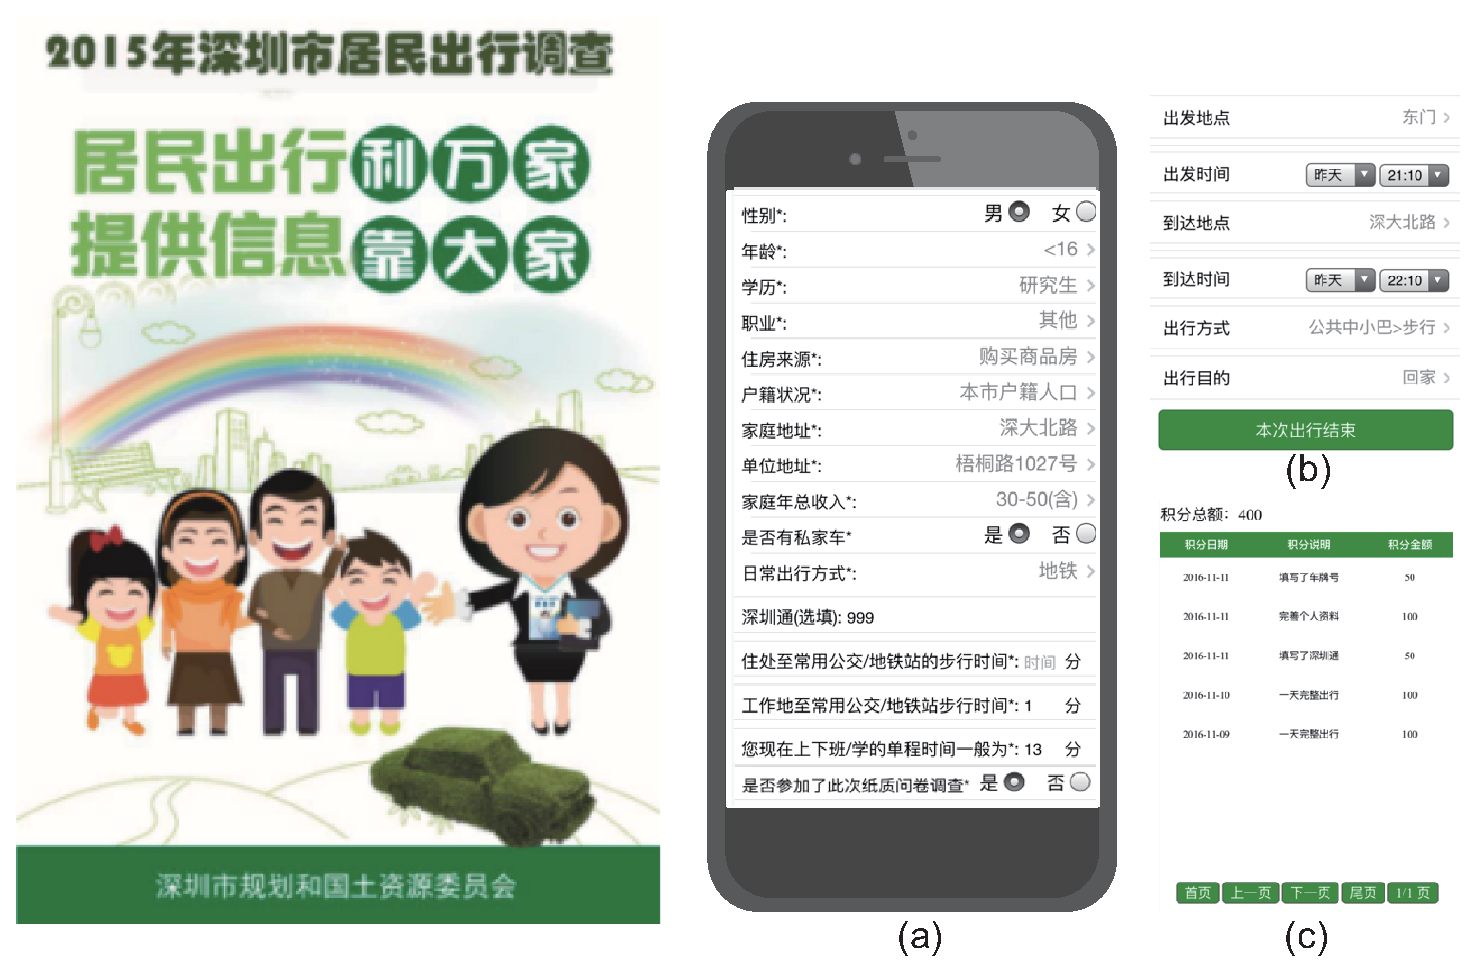
\includegraphics[width=\columnwidth]{pictures/survey_app}
 \caption{Census Interface: (a) personal characteristics collecting page; (b) trips collecting page; (c) credit system page}
 \label{fig:app}
\end{figure}

In this work, we perform the census survey in Shenzhen, which is one of the most modern metropolia in China. The experiment is deployed on Wechat, a widely used social media application. Figure~\ref{fig:app} shows the data collecting interfaces. Each individual hands in his or her personal characteristics. For privacy issue, all detailed personal information are desensitized to categorical levels (Figure~\ref{fig:app}(a)).

\begin{figure}[htb!]
 \centering % avoid the use of \begin{center}...\end{center} and use \centering instead (more compact)
 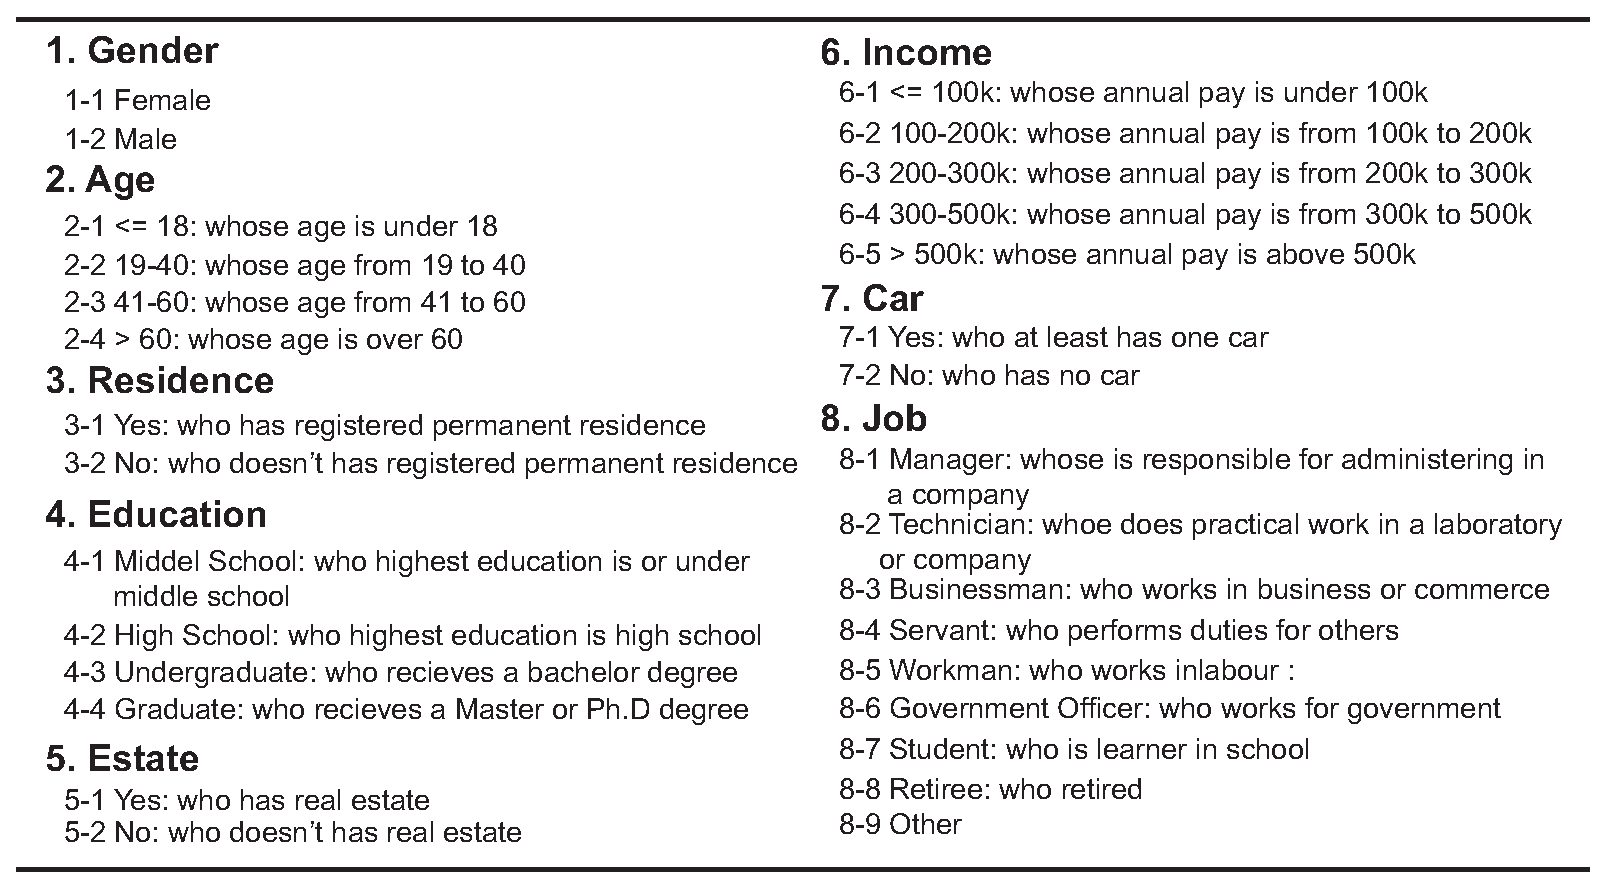
\includegraphics[width=\columnwidth]{pictures/data_over}
 \caption{Profile of Individual: eight individual characteristics enrich the analysis of mobility patterns}
 \label{fig:data_over}
\end{figure}


\textbf{Individual Characteristics} Figure~\ref{fig:data_over} lists the \textit{eight domains}, including social, economic and demographic aspects, to give a generalized description of the individual characteristics. The profile will serve as the ingredients for the analysis of mobility patterns over diverse individuals.

\textbf{Traveling Trips} Besides to those individual characteristics, each individual can upload dynamic traveling trips (Figure~\ref{fig:app}(b)). Each trip requires the information of \textit{start/end location}, \textit{start/end time}, \textit{traveling purpose}. To encourage the trip uploading, a credit system retains the contribution of individuals on trips and rewards the volunteers with the top credits (Figure~\ref{fig:app}(c)).


\subsection{Basic Statistics of Data}

Over the releasing time period from \m{2015-11 to 2016-01}, 21435 individuals (48\% females and 52\% males) were reached and \m{229155} trips are collected. Each volunteer contributes \m{11} trips average.

Our case-study data is confined to a small proportion of Wechat users who opt to contribute their information and trips.
Considering the caveat that self-selecting individuals are most unlikely to represent any clearly defined population~\citep{Longley2015}, we performed a series of preliminary statistics to check whether it is rich enough to represent a wide range of the population in the city.

\begin{figure}[htb!]
 \centering % avoid the use of \begin{center}...\end{center} and use \centering instead (more compact)
 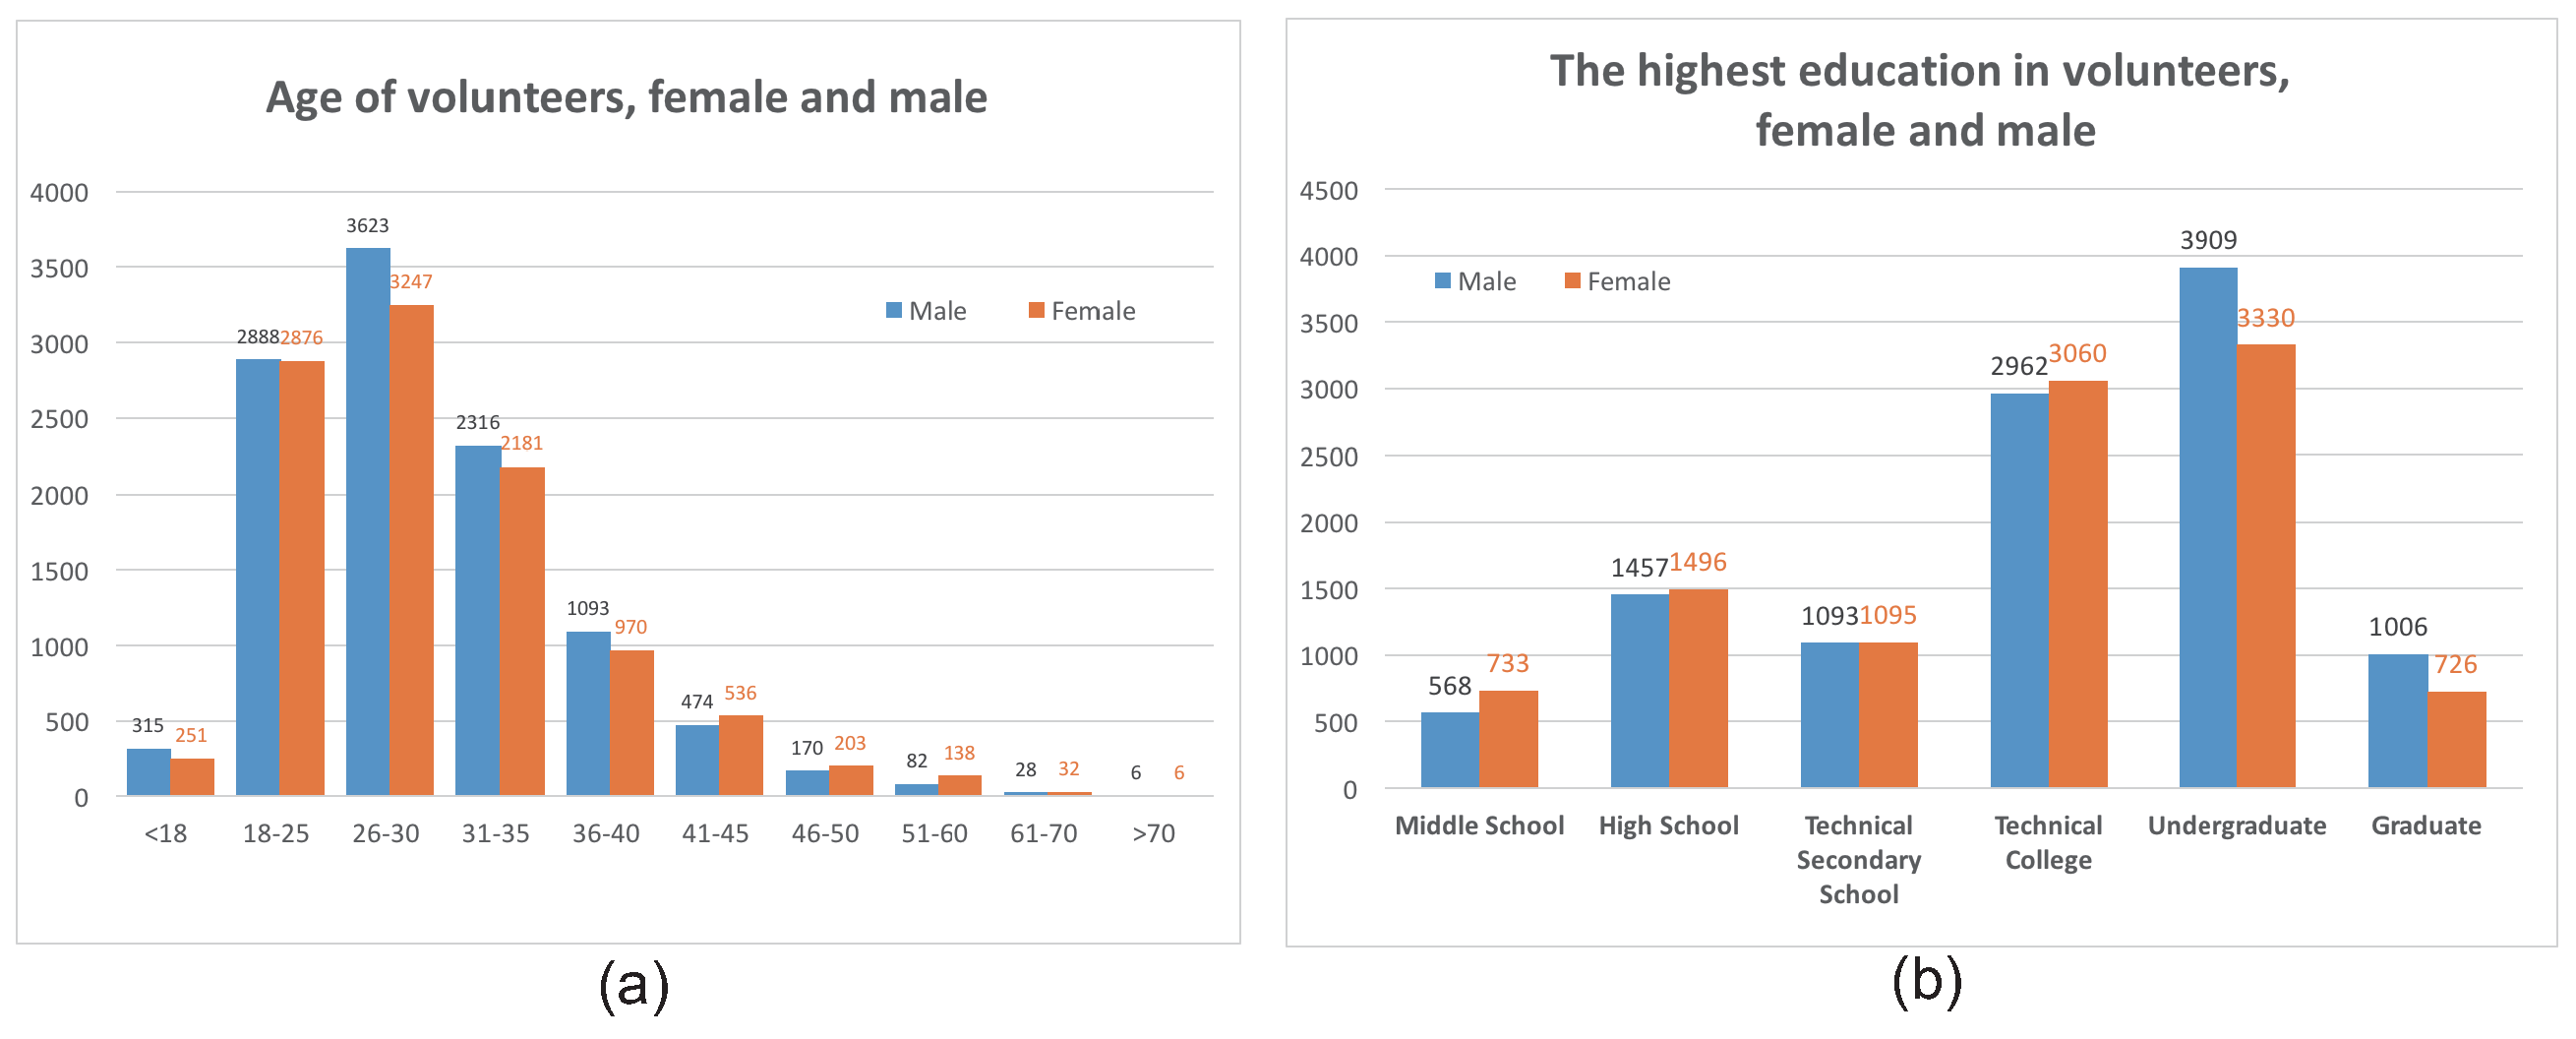
\includegraphics[width=\columnwidth]{pictures/data1}
 \caption{Age and Education Distribution: (a) age; (b) education}
 \label{fig:data_age_edu}
\end{figure}

Figure~\ref{fig:data_age_edu} gives the distribution of age and education over the population. It shows that samples cover a wide range of ages, dominating between 18 to 45. There is also a few records pertaining to individuals below the age of 18 or above 70. The distribution follows the fact that Shenzhen is a city where the majority is young people. According to the 2015 Annual Census Statistics report\footnote{http://www.sztj.gov.cn/xxgk/tjsj/pcgb/201606/t20160614\_3697000.htm}, people aging 15-64 occupy 83.23\% and the median age is 31.5. Figure~\ref{fig:data_age_edu} gives the distribution of education levels, ranging from low to high. The technical college and university dominate the samples at the 61\% occupancy rate.

\begin{figure}[htb!]
 \centering % avoid the use of \begin{center}...\end{center} and use \centering instead (more compact)
 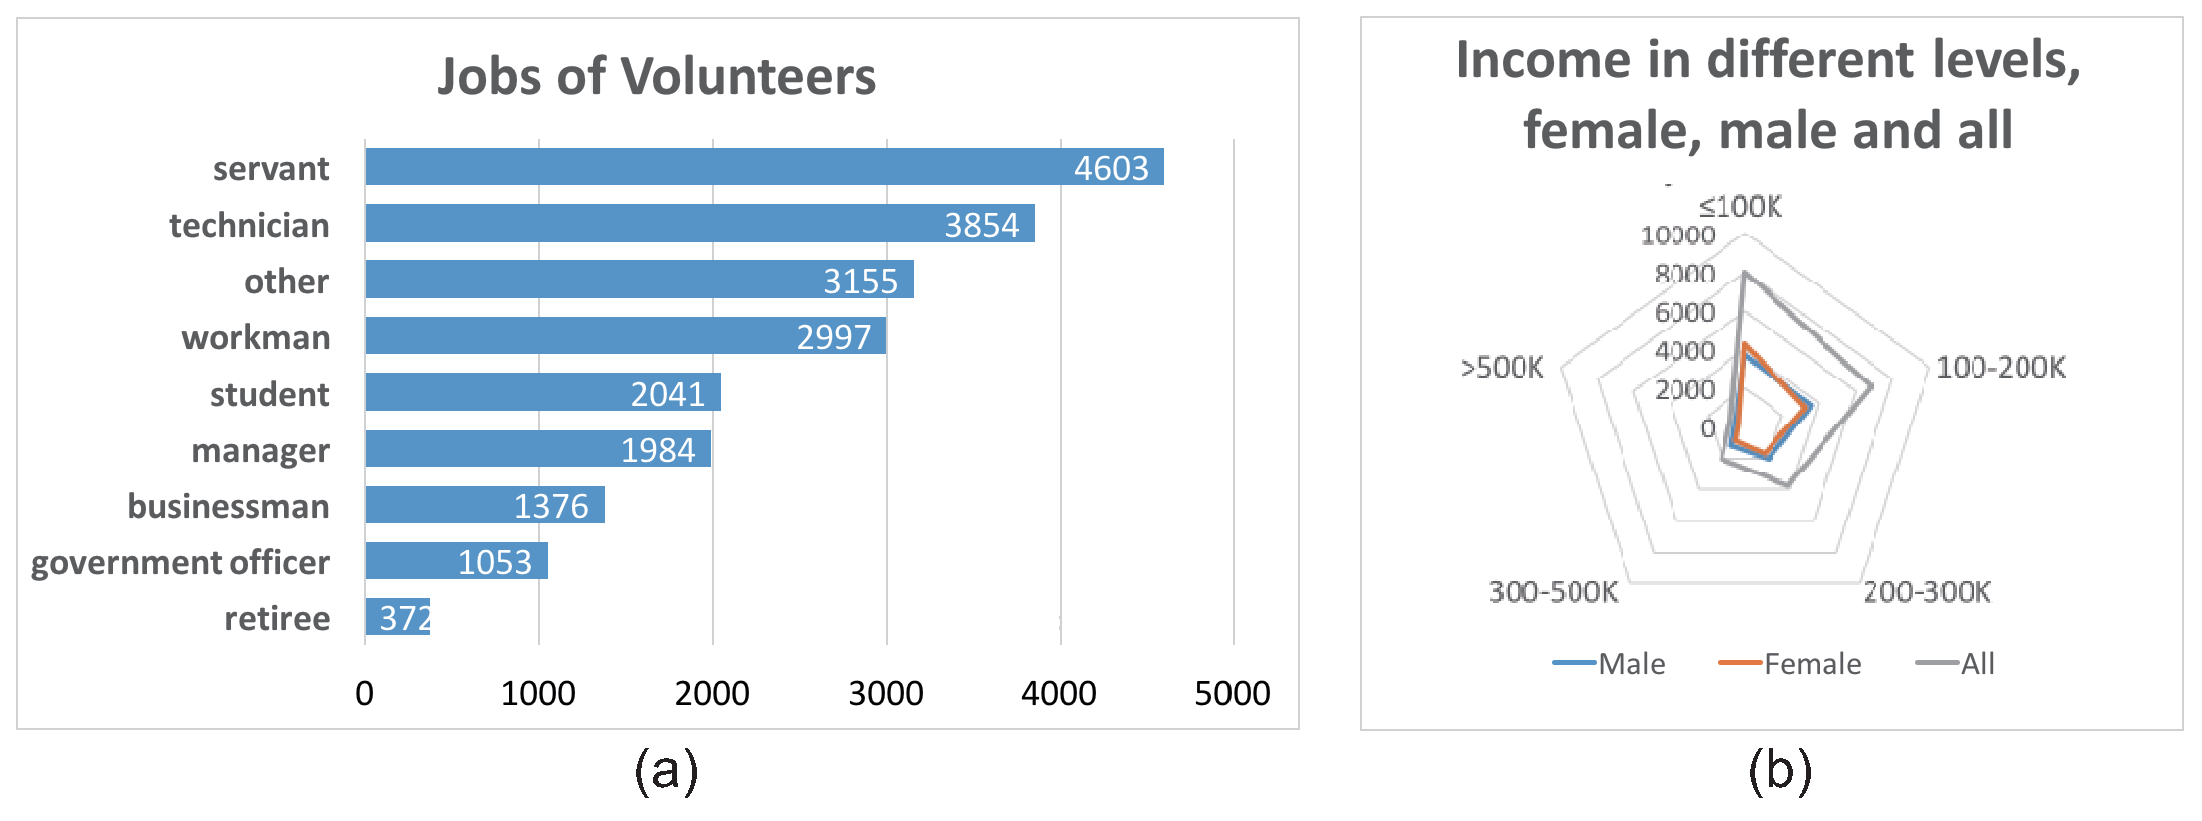
\includegraphics[width=\columnwidth]{pictures/data2}
 \caption{Job and Income Distribution: (a) job; (b) income}
 \label{fig:data_job_inc}
\end{figure}

Figure~\ref{fig:data_job_inc}(a) shows the job types of sampled individuals, who are servants, workers, officers, businessmen and so on. The covering of jobs is pretty wide. Figure~\ref{fig:data_job_inc}(b) gives the radar diagram of the annual pay. The majority get paid below 200 000. Individuals with higher salary are also reached in our census.

\begin{figure}[htb!]
 \centering % avoid the use of \begin{center}...\end{center} and use \centering instead (more compact)
 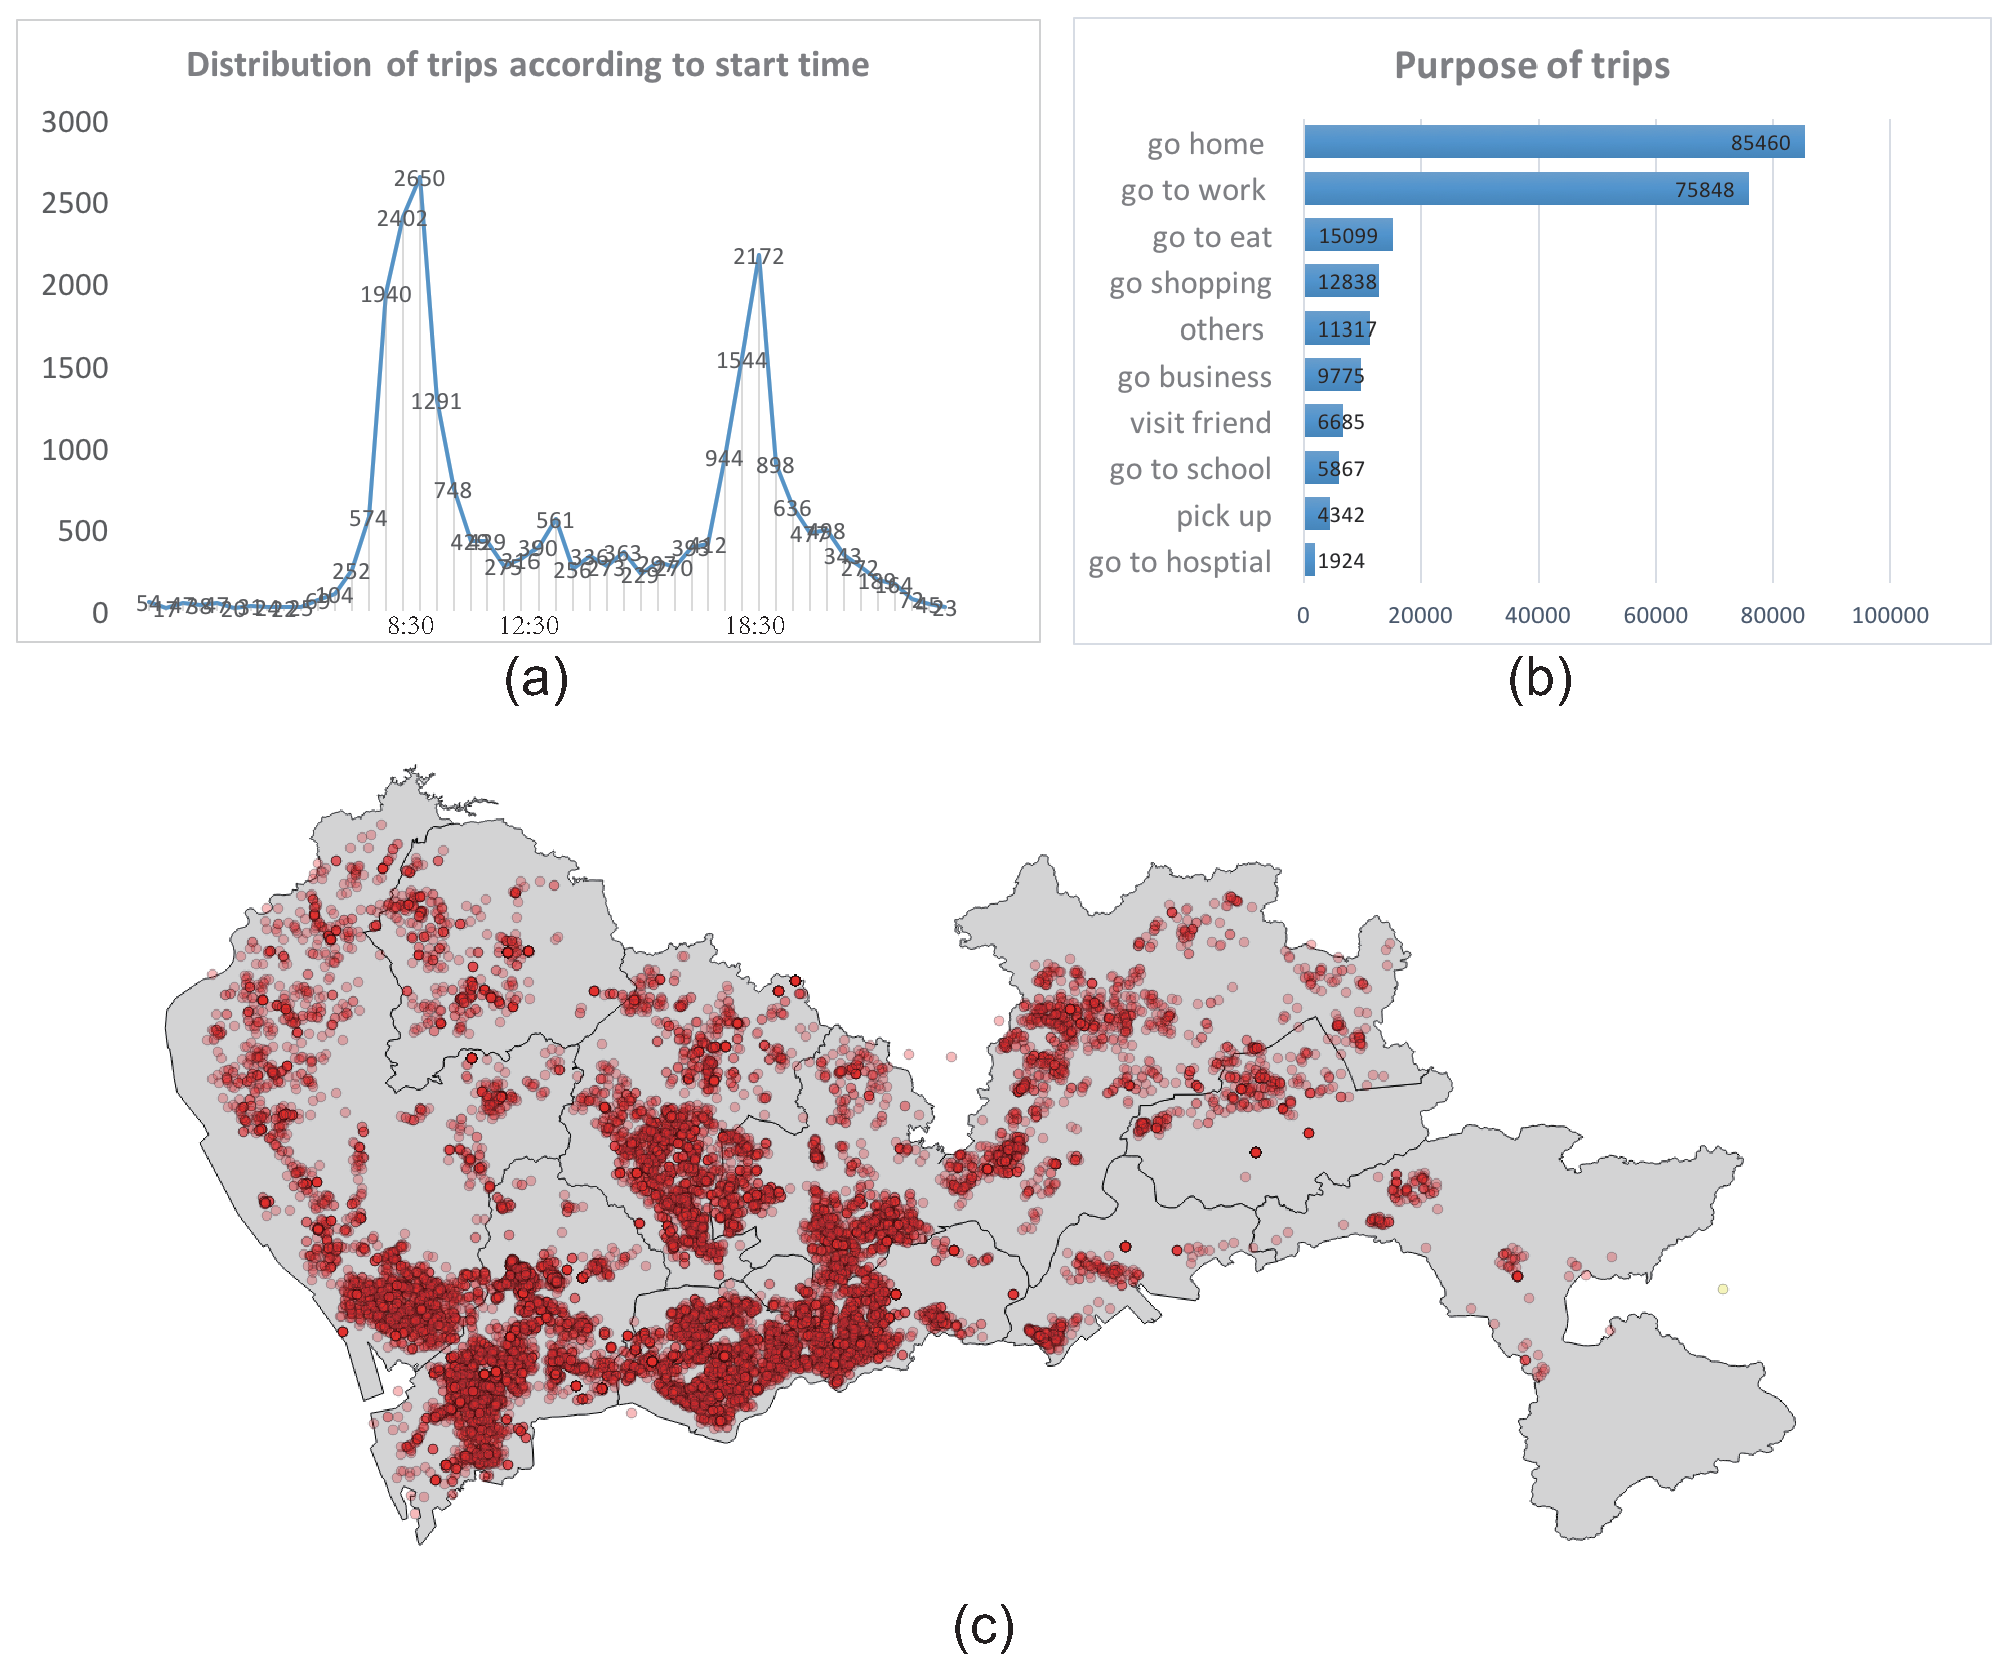
\includegraphics[width=\columnwidth]{pictures/data3}
 \caption{Statistics of Trips: (a) start time of trips; (b) purpose of trips; (c) distribution of origins/destinations }
 \label{fig:data_geometry}
\end{figure}

Figure~\ref{fig:data_geometry} shows the basic statistics related to trips. In Figure~\ref{fig:data_geometry}(a), the active traveling time (here, we take the start time as the representative of active time) follows the common knowledge of urban life. There are obvious morning and late afternoon peaks. Figure~\ref{fig:data_geometry}(b) gives the counting of different traveling purposes. 95\% trips are tagged with clear raveling purpose in the data. 33\% are going home and 37\% are going to work. Besides this kind of routine traveling, there are also substantial trips such as going shopping, going the hospital, etc. Figure~\ref{fig:data_geometry}(c) shows the spatial distribution of the origins and destinations. It is found that more dots are located in Futian and Nanshan districts, the city's heart than the surrounding areas. This is consistent to Batty's exposition of the focus of city networks and interaction patterns~\citep{batty2013new}.

Because there is always inevitable bias inherent in fully representing the ground truth of the population, the preliminary statistical analysis shows positive sign of a relatively even sampling of the population.

\section{Overview}
By communicating with domain expert, we summarize the analytic tasks identified from the interviews of domain experts. Aimed at these tasks, we derive design considerations and introduce the workflow of the proposed visual analytics system.

\subsection{Background}

For understanding how to express spatial attractiveness, we have several interviewers with an expert in GIS who works on human mobility and urban informatics. The experts pointed out that the study of social-spatial interactions has become more important with big and open data evolved in. Instead of evaluated by static indicators, such as the characteristics of the spatial facilities, spatial attractiveness can be evaluated dynamically with human movement data. People have their own preferences when they go out for a specific purpose. It reflects the attractiveness of the place they selected. When the research scale is expanded into city-scale, whether spatial attractiveness is similar of the citizens with similar social characteristics. However, for GIS researchers, there is no efficient and effective methods which help to explore spatial attractiveness, citizens with multiple social characteristics, and their relationships. After several rounds of interviews with experts, we summarize the main analysis criteria below:

\begin{itemize}
\item \textit{Multiple social characteristics} 

\item \textit{Spatial attractiveness} In urban planning and GIS, the definitions of spatial attractiveness is based on gravity model\wqc{add refer}. It means the more distant the less attractiveness. Hence, both the quantity of people attracted and movement distances are two crucial concepts to be explored.

\item \textit{Attractiveness diversity} In urban planning, functional area is an important concept. When the area has more functions, for people here, their living requirements are more easily met, the attractiveness diversity of the area is higher.  ......

\end{itemize}

\subsection{Tasks}
The exploration of core concepts above are resolved further with following tasks... to align the analysis of mobility patterns with individual characteristics. Before diving into the design of the system, introduce the couple of specifical tasks the system intended for.

\begin{itemize}
\item \textit{Task 1: Identify the group with specific individual characteristics\wqc{What kind of citizens tend to be attracted?}}: to get groups of people with common or close attributes, to explore the correlation among individual characteristics.
\item \textit{Task 2: What is the correlation between space and citizens? (Spatial Attractiveness)} to understand... group of citizens are attracted to different places, e.g., to know the similarities and differences between different groups in their mobility patterns, to investigate the relationship between movement and individual characteristics.
\item \textit{Task 3: What is the detailed properties of attractive differences?} ... How many citizens are extracted, the origins (Where do the attracted citizens come from?) What is the attractive differences over groups?
\end{itemize}


\subsection{Design Considerations}

With these three tasks, we derive following design considerations:

\begin{itemize}
\item \textit{Intuitive perception of an individual as an organic complex (C1)}: the system should make use of users' daily life experience in knowing people to provide intuitive visualization, instead of the lifeless representation by number. The visual design needs to help end-users to pick desirable ones from the mass.
\item \textit{Good overview of the multivariate individuals (C2)}: following the visual analytics manta by Shneiderman~\citep{RN459}, it is very important to provide a good overview of all the individuals then the users know where to explore.
\item \textit{Effective multivariable cross-filter for individual characteristics (C3)}: there are eight domains to describe an individual. The system is supposed to provide a straight-forward way for easy filtering by the eight criteria.
\item \textit{Compact visualization of mobility patterns in the constraint of spatial space (C4)}: the analysis of mobility patterns not only includes the conventional spatial and temporal dimensions, but also other abstract dimensions, e.g., travel purpose, visiting frequency, etc. The system should handle a compact layout to support the easy correlation between spatial and abstract information.
\item \textit{Flexible interactions to explore the mobility patterns either within one group or between groups (C5)}: to support the comparison among groups, \textit{Task 3}, the system should maintain flexible interactions which allow the end-users to explore freely.
\end{itemize}


\section{Visual Design}
\begin{figure}[htb!]
 \centering 
 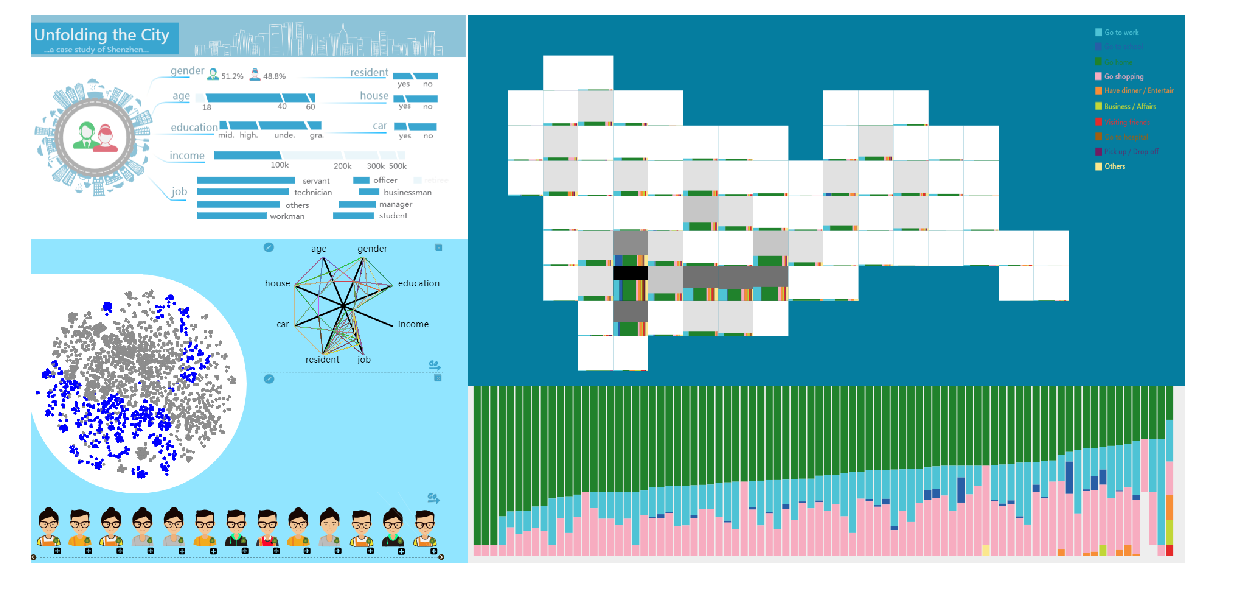
\includegraphics[width=\linewidth]{pictures/interface53}
 \caption{\wqc{to be edit. System Interface: (a) an interactive infographics provides the basic statistic facets of individuals; (b) View1: a XXXX visualization gives an overview of individuals, where the similarity in high dimensional space is preserved in 2D space; (c) View2: data-driven profiles support users with organic individual perception; (d) View3: map view for movement of the chosen group; (e) View4: for ranking or comparison; (g) View5: top N kinds of citizens with social characteristics.}}
 \label{fig:interfaceDraft}
\end{figure}

With those design considerations described before, we develop a visual analytics system as Figure~\ref{fig:interfaceDraft} shows. It composes of individual panel (the left part) for individuals (\textit{Task 1}) and spatial panel (the right part) for the mobility pattern (\textit{Task 2 and 3}). In the individual panel, interactive infographics, t-SNE visualization, and data-driven social profiles support users to narrow the scope down to groups of individuals with interested characteristics. With the chosen group of individuals, spatial attractiveness is visualized and explored in a map view with the \wqc{no name} glyph we designed. 

\subsection{Social Profile Visualization}
To express the multiple dimensional social characteristics, we use three scales: bar glyph for all citizens, octagon glyph for a group of persons, and cartoon glyph for one person.

\paragraph{Bar Glyph}
As shown in Figure~{\ref{fig:interfaceDraft}}(a), bar glyphs are used to encode quantitative relationships. For each characteristic, we compute the quantity and the percentage of each type, and encode it in the length of the bar. Interaction is also bound. When clicking a bar, filtering will be done, and the filtering result will be used in grouping phrase.

\paragraph{Octagon Glyph}
Glyph-based visualization~\cite{borgo2013glyph} is the form of visual design to compose multivariable into a collection of unified visual symbols, known as a glyph. A glyph is intended for quick understanding and aligned comparison. 


\paragraph{Cartoon Glyph}
Among glyph design, Chernoff Face (Chernoff, 1973) represents data variables by the different features of a cartoon face. Following the idea of Chernoff Face, we design a type of glyph, a graphical representation of people with specific individual characteristics. The idea behind using faces is that humans easily recognize faces and notice small changes without difficulty (C1). Those visual profiles are intended for intuitive visual understanding, from abstract to concrete and semantic understanding, to support users to target the interested individual groups effectively.

\begin{figure}[htb!]
 \centering 
 \includegraphics[width=0.6\columnwidth]{pictures/cartoonglyph}
 \caption{***********************}
 \label{fig:cartoon}
\end{figure}

Figure~\ref{fig:cartoon} shows the legend for the user profile. The eight domains are encoded by vi- sual symbols and organically organized in a human figure. There are basically three types of variables to drive the figure, i.e., the numeric, categorical and boolean ones. For numeric attributes such as income and education levels, visual symbol keeps consistent design but with changing visual variation, such as size, thickness. For the categorical attributes such as job, visual symbols are designed separately for better semantic meaning. For the boolean at- tribute like car, house, a symbol is designed to indicate its existence. With this consideration, the domains are designed as follows:

\begin{itemize}
\item \textbf{Gender} the gender is visually mapped to the hairstyle of the avatar.
\item \textbf{Age} age is implied by the decoration on the hair. For the elder above 70, the hair is dyed to gray. For the youth beneath 18, a hair decoration is adapted for the different hairstyles of girls and boys.
\item \textbf{Education} The thickness of eyeglasses is used to indicate the different levels of education.
\item \textbf{Job} The clothes is designed to imply the job of the individual. There are 9 types of clothes.
\item \textbf{Belongings} for real estate, car, residential license are considered as the belongings to the individual, so we design each of them as an add-on decoration to imply whether the individual has it or not.
\item \textbf{Income} a money symbol is used to represent the income, whose size encodes the income level. The more money an individual earns, the larger the symbol is.
\end{itemize}

\begin{figure}[htb!]
 \centering % avoid the use of \begin{center}...\end{center} and use \centering instead (more compact)
 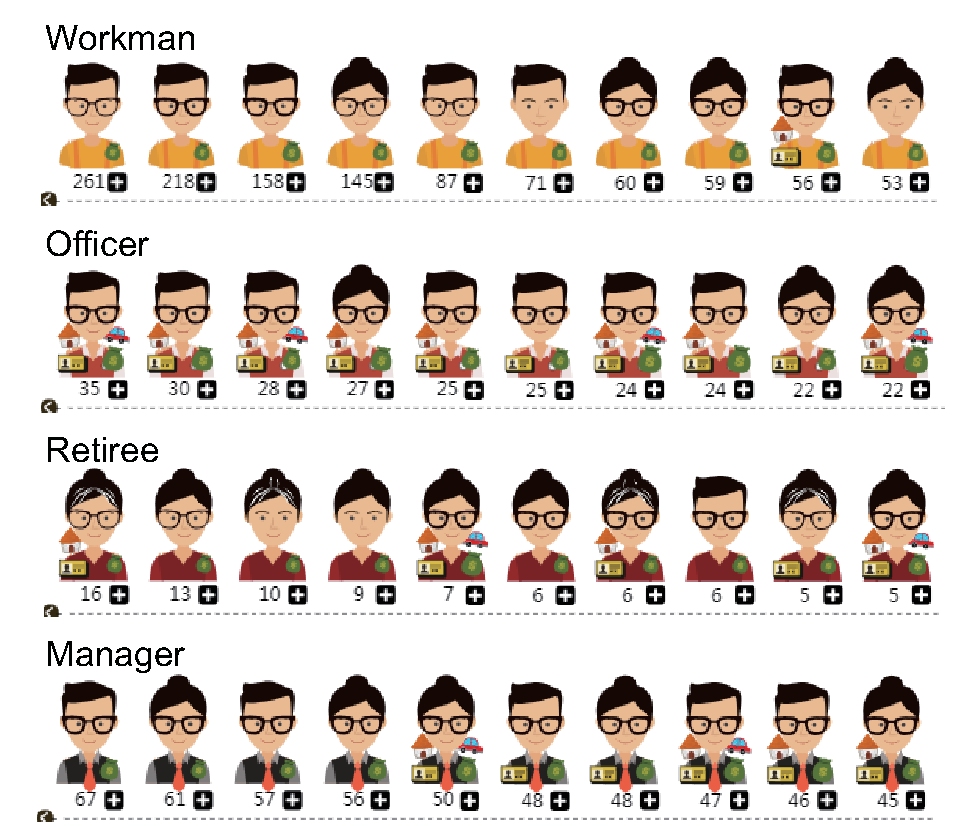
\includegraphics[width=0.6\columnwidth]{pictures/design_example}
 \caption{Representative figures with the top 10 largest population in four jobs}
 \label{fig:div_example}
\end{figure}

With the visual mapping, the profile varies from individual to individual. By concretizing the attributes which otherwise is too abstract to percept, users can scan and search for interesting target effectively. Figure~\ref{fig:div_example} lists the figures with the top 10 largest population in some job. The textual number beneath indicates the population. It is found that the majority of workmen earn a low salary and most of them have no residential license. On the contrary, for the officers, all of them have the residential license and most of them have a house. Some of the retired people are in old age. Most of the managers are at undergraduates, even graduates.




\subsection{T-SNE Projection of Individuals}

\begin{figure}[htb!]
 \centering % avoid the use of \begin{center}...\end{center} and use \centering instead (more compact)
 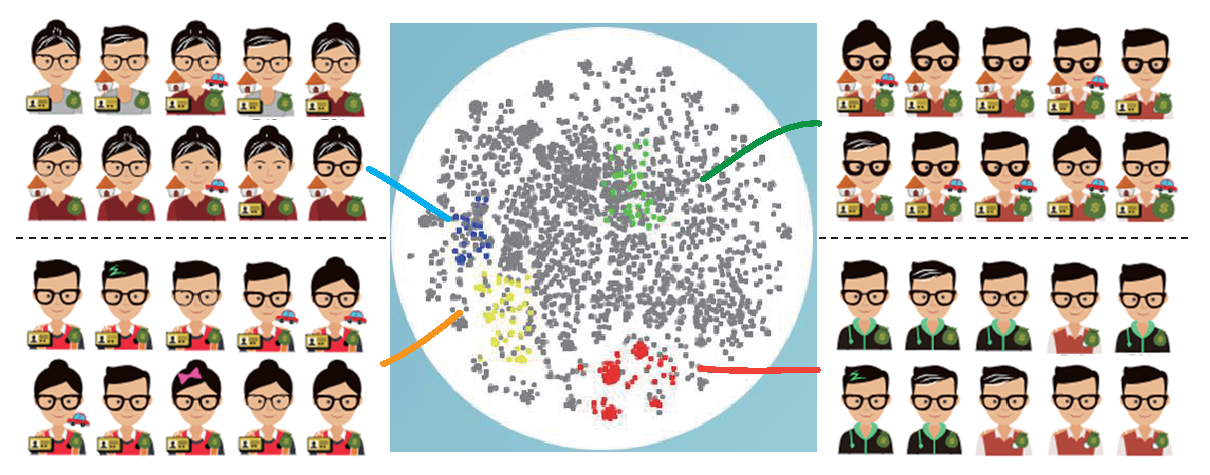
\includegraphics[width=\columnwidth]{pictures/tsne}
 \caption{t-SNE project with four groups of the interest: (a) t-SNE project }
 \label{fig:tsne}
\end{figure}

In our case, each individual can be denoted as a vector $x_i$ with eight factors, and we get high dimensional data set $X={x_1, x_2, ..., x_n}$. The dimensionality reduction techniques are to preserve the local structure of high dimensional data in low dimensional space, which are efficient approaches to provide a good overview of the multivarible individuals (\textit{C2}). We adapt t-SNE project~\citep{maaten2008visualizing} to project $X$ as two-dimensional dots $Y={y_1, y_2, ..., y_n}$. One of steps in t-SNE is to compute the conditional probabilities to represent the similarity based on the distance between high dimenional datapoints. The conditional probability $p_{j\mid i}$ between $x_j$ and $x_i$ is given by:

\begin{equation}
p_{j\mid i} = \frac{exp({\left \| x_i - x_j \right \|}^2/2\alpha_i ^{2})}{\sum _{k\neq i}exp({\left \| x_i - x_k \right \|}^2/2\alpha_i ^{2})}
\end{equation}

where $\alpha_i$ is the variance of the Gaussian that is centered on $x_i$. Specifically in our context, the high-dimensional Euclidean distances $\left \| x_i - x_j \right \|$ between $x_i$ and $x_j$ needs to be adpated the numerical and categorical characteristics. Characteristics such as age, income, are numerical and comparable, so the difference exactly explains when they are different. But the other characteristics, i.e. job, real estate, car, residential, are ordinal. There is not the numeric order. For example, the job distance from a manager to a businessman and a workman is not comparable, which is considered the same distance, i.e., set to 1.


As Figure~\ref{fig:tsne}shows, all 21435 volunteers are embedded in the 2D view, where the closer two dots are, the more similar they are in the eight characteristics. Figure~\ref{fig:tsne} exemplifies four features groups of dots in a neighbor.

Multiple views of abstract view, t-SNE protection, and semantic data-driven profile visualization are coordinated in a Cross-filter machinesm~\citep{Weaver2010}. It allows end-users to interactive drill-down into individuals with interested characteristics from multiple perspectives(\textit{C3}). Starting from the abstract criterion constraints, the scope of interest is narrowed down to individuals with(out) certain characteristics. And then further cross-filtering with semantically visual profiles can be performed to check the combination of 8 characteristical variables.


\subsection{Location-based multidimensional grid visualization}
We design a kind of glyph to express a high-dimensional travel indicators. It will be embed in the map view. 

The elements can be represented in the glyph:
\begin{itemize}
  \item value
  \item distribution
  \item proportion
\end{itemize}



\section{Experts Feedback}

\lmc{Add a section to introduce the domain experts' feedback}
\lm{We interview XX domain experts from the GIS field. XX of them are with ... The procedure went as following. We first introduce them the system an...}

\section{Case studies}

In this section, we apply the method described above to study the case of Shenzhen. We introduce the several cases to demonstrate the usage and effectiveness of the system.


\subsection{Case 1: Group by similar social characteristics}
\paragraph{Use bar and tsne to find four groups. figure to show groups.}
\paragraph{Their home locations and basis travel features.}


\subsection{Case 2: Spatial Attractiveness}
\paragraph{Select two groups, and target purpose. figure to compare spatial attractiveness.}
\paragraph{click a grid, show OD. figure}


\subsection{Case 3: Diversity of spatial attractiveness}
\paragraph{Select group, figure to show diversity.}
\paragraph{ranking, figure}
\paragraph{two groups to compare, figure}


\section{Discussion and Conclusion}




%\begin{acknowledgements}
%If you'd like to thank anyone, place your comments here
%and remove the percent signs.
%\end{acknowledgements}

% BibTeX users please use one of
\bibliographystyle{spbasic}      % basic style, author-year citations
%\bibliographystyle{spmpsci}      % mathematics and physical sciences
%\bibliographystyle{spphys}       % APS-like style for physics
\bibliography{main}
%\bibliography{test}


\end{document}
% end of file template.tex

